% Präambel: \usepackage{tikz} (hast du schon)

\definecolor{qcHell}{HTML}{4A8CD6}
\definecolor{qcMittel}{HTML}{0057B0}
\definecolor{qcDunkel}{HTML}{002868}
\definecolor{qcNadel}{HTML}{525A78}
\definecolor{qcHintergrund}{HTML}{E0F0FF}

% Ein Ringsegment: Startwinkel, Endwinkel, Farbe
\newcommand{\qcSegment}[3]{%
  \fill[#3] ({4*cos(#1)},{4*sin(#1)}) arc[start angle=#1, end angle=#2, radius=4]
            -- ({2.6*cos(#2)},{2.6*sin(#2)}) arc[start angle=#2, end angle=#1, radius=2.6]
            -- cycle;
}

\newcommand{\qcTacho}{%
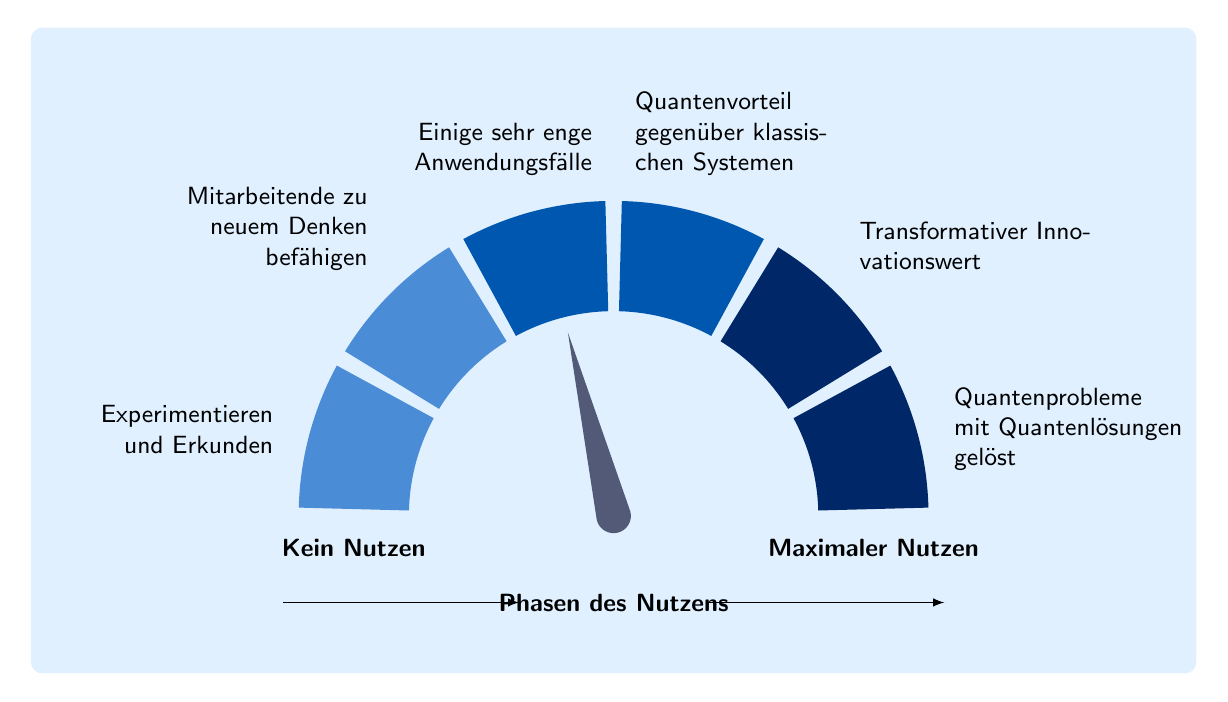
\begin{tikzpicture}[>=latex, font=\sffamily\small, lab/.style={text width=3cm}]

  % Hintergrund (optional, Zeile entfernen für transparenten Hintergrund)
  \fill[qcHintergrund, rounded corners=4pt] (-7.4,-2) rectangle (7.4,6.2);

  % Segmente mit 3° Lücke
  \qcSegment{178.5}{151.5}{qcHell}
  \qcSegment{148.5}{121.5}{qcHell}
  \qcSegment{118.5}{91.5}{qcMittel}
  \qcSegment{88.5}{61.5}{qcMittel}
  \qcSegment{58.5}{31.5}{qcDunkel}
  \qcSegment{28.5}{1.5}{qcDunkel}

  % Nadel (Spitze bei 104°, also im dritten Segment)
  \fill[qcNadel] ({2.4*cos(104)},{2.4*sin(104)})
      -- ({0.22*cos(14)},{0.22*sin(14)})
      arc[start angle=14, end angle=-166, radius=0.22] -- cycle;

  % Beschriftung der Segmente
  \node[lab, anchor=east, align=right]       at (-4.2,1.1)  {Experimentieren und Erkunden};
  \node[lab, anchor=south east, align=right] at (-3.0,3.0)  {Mitarbeitende zu neuem Denken befähigen};
  \node[lab, anchor=south east, align=right] at (-0.15,4.2) {Einige sehr enge Anwendungsfälle};
  \node[lab, anchor=south west, align=left]  at (0.15,4.2)  {Quantenvorteil gegenüber klassischen Systemen};
  \node[lab, anchor=south west, align=left]  at (3.0,3.0)   {Transformativer Innovationswert};
  \node[lab, anchor=west, align=left]        at (4.2,1.1)   {Quantenprobleme mit Quantenlösungen gelöst};

  % Endpunkte und Phasenachse
  \node[font=\sffamily\small\bfseries] at (-3.3,-0.4) {Kein Nutzen};
  \node[font=\sffamily\small\bfseries] at (3.3,-0.4)  {Maximaler Nutzen};
  \draw[->] (-4.2,-1.1) -- (-1.2,-1.1);
  \draw[->] (1.2,-1.1)  -- (4.2,-1.1);
  \node[font=\sffamily\small\bfseries] at (0,-1.1) {Phasen des Nutzens};

\end{tikzpicture}%
}